\documentclass{templateNote}
\usepackage{tcolorbox}
\usepackage{hyperref}
\usepackage{amsmath}
\usepackage{amssymb}
\usepackage{soul}
\usepackage{circuitikz}


\lstdefinestyle{mystyle}{
    backgroundcolor=\color{gray!10}, % Color de fondo
    commentstyle=\color{green},
    keywordstyle=\color{blue},
    numberstyle=\tiny\color{gray},
    stringstyle=\color{red},
    basicstyle=\ttfamily\footnotesize, % Estilo básico del texto con tamaño grande
    breakatwhitespace=false, % No romper en espacios en blanco
    breaklines=true, % Romper líneas largas
    captionpos=b, % Posición del título
    keepspaces=true, % Mantener espacios
    numbers=left, % Numeración a la izquierda
    numbersep=5pt, % Separación de los números
    showspaces=false, % No mostrar espacios
    showstringspaces=false, % No mostrar espacios en cadenas
    showtabs=false, % No mostrar tabulaciones
    tabsize=2 % Tamaño de tabulación
}

\lstset{style=mystyle}

% \textbf{Código ensamblador MIPS}
%     \begin{lstlisting}
% add t, b, c # t = b + c
% sub a, t, d # a = t - d
%     \end{lstlisting}


\begin{document}
\imagenlogoU{img/logoNGMFormal_sinF.png}
\linklogoU{https://github.com/NicoGomezM} 
% \imagenlogoD{img/logo-ubb-txt-face.png} 
\titulo{Apunte 1}
\asignatura{Inteligencia Artificial}
\autor{
    \indent
    Nicolás {Gómez Morgado}
}


\portada
\margenes 
\tableofcontents
\newpage



\section{Importante}
\noindent Evaluaciones 2,3 y 4 en grupos (máximo 2-3 personas), 1 individual.

\begin{enumerate}
    \item 13 sept
    \item 4 oct
    \item 30 oct
    \item 20 dic
\end{enumerate}

\begin{itemize}
    \item Herramientas:
    \begin{itemize}
        \item Phyton
        \item Google colab
    \end{itemize}
\end{itemize}

\noindent\textbf{Tensor:} Vector con otro nombre.

\newpage
\section{Inteligencia Artificial}
\subsection{Introducción}
La inteligencia artificial es una rama de la informática que se encarga de desarrollar algoritmos y programas que permiten a las computadoras realizar tareas que requieren de la inteligencia humana. En este momento ya se ha logrado incluir la inteligencia artificial en muchos aspectos de la vida cotidiana, como por ejemplo en los asistentes virtuales, en los sistemas de recomendación, en los vehículos autónomos, en la medicina, en la industria, entre otros. Por lo cual un concepto que hace no mucho parecía de ciencia ficción, hoy en día es una realidad.

\subsection{Conceptos fundamentales}
Tiene como objetivo desarrollar algoritmos que permitan a las maquinas aprender de la experiencia y mejorar su rendimiento en tareas específicas. Para esto se utilizan técnicas de aprendizaje automático, que son un subconjunto de la inteligencia artificial.
\\\\\noindent
\textbf{Tipos de inteligencia artificial:}
\begin{itemize}
    \item \textbf{IA débil:} Realiza tareas especificas y limitadas.
    \item \textbf{IA fuerte:} Realiza tareas generales y complejas mas asociadas al pensar humano.
\end{itemize}
\noindent
\textbf{Ética en la IA:} Que tipos de datos se utilizan, como se utilizan, que impacto tiene en la sociedad, etc. El objetivo es que la IA sea ética y presente algún tipo de sensibilidad social. A pesar de que la IA no tiene conciencia, si puede tener un impacto en la sociedad y siempre va a presentar errores, por lo que es importante tener en cuenta la ética en la IA.

\begin{center}
    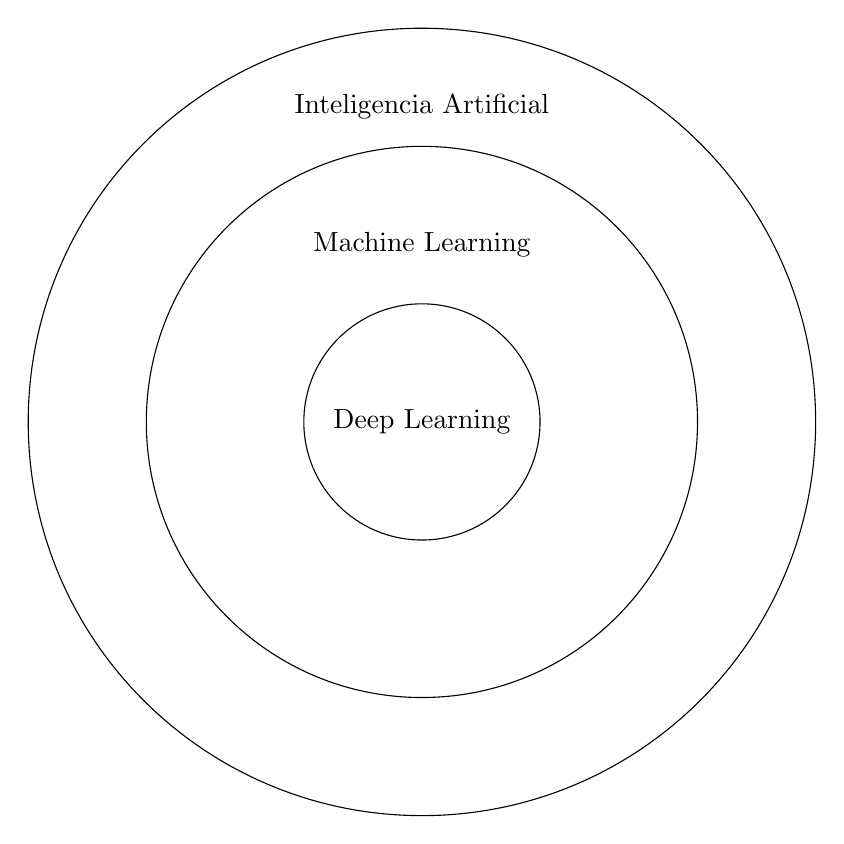
\begin{tikzpicture}
        % Outer circle
        \draw (0,0) circle (5cm);
        
        % Inner circles
        \draw (0,0) circle (3.5cm);
        \draw (0,0) circle (1.5cm);
        % \draw (0,0) circle (0.5cm);
        
        % Labels
        \node at (0,4) {Inteligencia Artificial};
        \node at (0,2.25) {Machine Learning};
        \node at (0,0) {Deep Learning};
    \end{tikzpicture} 
\end{center}

\begin{tcolorbox}[colback=gray!5!yellow!40,colframe=gray!75!black]
    \noindent\textbf{Primeras ''Inteligencias Artificiales'' a crear van a estar enfocadas en Machine Learning.}
\end{tcolorbox}

\noindent
\textbf{Elementos para el aprendizaje de la IA:} La IA requiere de fuentes de datos para entrenarse a si misma. Algunas fuentes de datos son:

\begin{itemize}
    \item kaggle
    \item sklearn
    \item visualdata.io
\end{itemize}


\noindent\textbf{Código Python para importar y usar librerías:}
\begin{lstlisting}
import numpy as np
import pandas as pd
import matplotlib.pyplot as plt 

# Cargar datos
data = pd.read_csv('data.csv')

# Visualizar datos
print(data.head())

# Graficar datos
plt.plot(data['x'], data['y'])
\end{lstlisting}

\newpage
\section{Matemáticas aplicadas a la IA}

\newpage
\section{Deep Learning}

\newpage
\section{Machine Learning}

\end{document}
